\documentclass[tikz,border=8pt]{standalone}
\usepackage{amsmath}
\usepackage{xcolor}
\definecolor{bg}{HTML}{171D2B}
\definecolor{accent}{HTML}{F7B538}
\definecolor{linecol}{HTML}{8FA3BF}
\usetikzlibrary{calc}
\pagecolor{bg}
\begin{document}
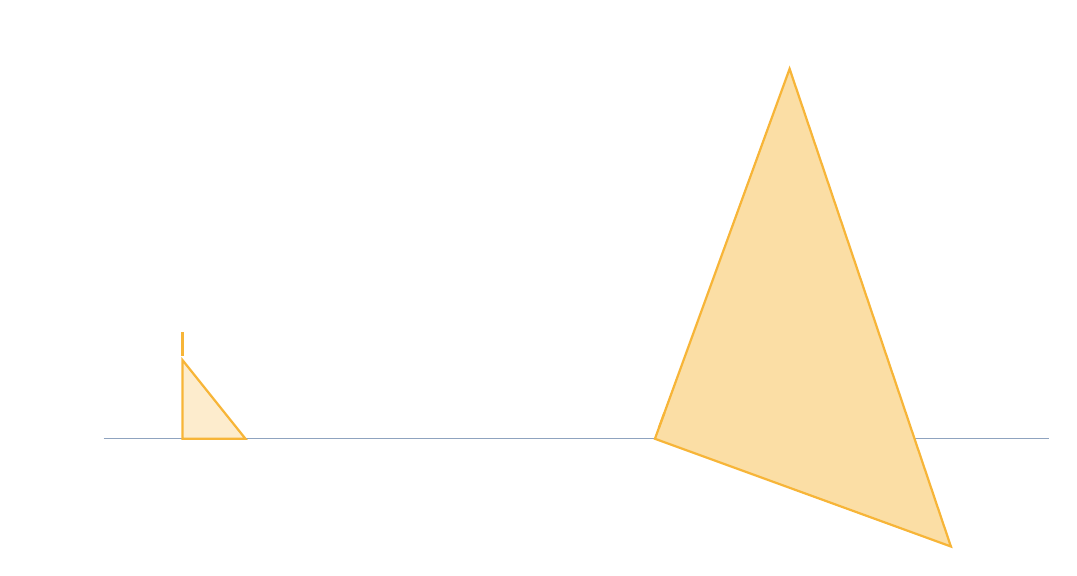
\begin{tikzpicture}[
  scale=1.0,
  text=white,
  every node/.style={text=white, font=\small},
  axis/.style={draw=linecol, thin}
]
  % garis tanah
  \draw[axis] (-1,0) -- (11,0);

  % Segitiga tongkat: tinggi 1, bayangan 0.8
  \coordinate (A) at (0,0);
  \coordinate (B) at (0,1);
  \coordinate (C) at (0.8,0);
  \draw[thick, draw=accent, fill=accent!25] (A) -- (B) -- (C) -- cycle;
  \draw[thick, accent] (0,1.05) -- (0,1.35);
  \node[left, align=right] at (0,1.2) {tongkat 1 m};
  \node[below] at (0.4,0) {80 cm};

  % Segitiga pohon: dikalikan k = 5, lalu diputar -20 derajat di sekitar pangkal
  \begin{scope}[rotate around={-20:(6,0)}]
    \coordinate (P) at (6,0);
    \coordinate (Q) at ($(P)+(0,5)$);
    \coordinate (R) at ($(P)+(4,0)$);
    \draw[thick, draw=accent, fill=accent!45] (P) -- (Q) -- (R) -- cycle;
    \draw[thick, accent] ($(P)!0.03!(Q)$) -- ($(P)+(0,0.35)$);
    \node[above left, align=right] at (Q) {pohon?};
    \node[below] at ($(P)!0.5!(R)$) {4 m};
  \end{scope}
\end{tikzpicture}
\end{document}
